\documentclass[10pt]{article}
\usepackage{amsmath} 
\usepackage{fontspec}
\usepackage[a4paper, margin=12mm]{geometry}
\usepackage{graphicx}
\usepackage{titlesec}
\usepackage{amsmath}
\usepackage{fancyhdr}
\usepackage{amsmath}
\usepackage{datetime}
\usepackage[hidelinks]{hyperref}
\usepackage[utf8]{inputenc}
\usepackage{booktabs}

\setmainfont{JetBrains Mono}
\setmainfont[NFSSFamily=dayrom]{JetBrains Mono}
\graphicspath{ {./images/} }

\DeclareSymbolFont{digits}{TU}{dayrom}{m}{n}
\AtBeginDocument{
	\DeclareMathSymbol{0}{\mathalpha}{digits}{`0}
	\DeclareMathSymbol{1}{\mathalpha}{digits}{`1}
	\DeclareMathSymbol{2}{\mathalpha}{digits}{`2}
	\DeclareMathSymbol{3}{\mathalpha}{digits}{`3}
	\DeclareMathSymbol{4}{\mathalpha}{digits}{`4}
	\DeclareMathSymbol{5}{\mathalpha}{digits}{`5}
	\DeclareMathSymbol{6}{\mathalpha}{digits}{`6}
	\DeclareMathSymbol{7}{\mathalpha}{digits}{`7}
	\DeclareMathSymbol{8}{\mathalpha}{digits}{`8}
	\DeclareMathSymbol{9}{\mathalpha}{digits}{`9}
}

% subsubsubsection
\titleclass{\subsubsubsection}{straight}[\subsection]
\newcounter{subsubsubsection}[subsubsection]
\renewcommand\thesubsubsubsection{\thesubsubsection.\arabic{subsubsubsection}}
\renewcommand\theparagraph{\thesubsubsubsection.\arabic{paragraph}} % optional; useful if paragraphs are to be numbered

\titleformat{\subsubsubsection}
{\normalfont\normalsize\bfseries}{\thesubsubsubsection}{1em}{}
\titlespacing*{\subsubsubsection}
{0pt}{3.25ex plus 1ex minus .2ex}{1.5ex plus .2ex}

\makeatletter
\renewcommand\paragraph{\@startsection{paragraph}{5}{\z@}%
	{3.25ex \@plus1ex \@minus.2ex}%
	{-1em}%
	{\normalfont\normalsize\bfseries}}
\renewcommand\subparagraph{\@startsection{subparagraph}{6}{\parindent}%
	{3.25ex \@plus1ex \@minus .2ex}%
	{-1em}%
	{\normalfont\normalsize\bfseries}}
\def\toclevel@subsubsubsection{4}
\def\toclevel@paragraph{5}
%\def\toclevel@paragraph{6}
\def\toclevel@subparagraph{6}
\def\l@subsubsubsection{\@dottedtocline{4}{7em}{4.5em}}
\def\l@paragraph{\@dottedtocline{5}{10em}{5em}}
\def\l@subparagraph{\@dottedtocline{6}{14em}{6em}}
\makeatother

\setcounter{secnumdepth}{4}
\setcounter{tocdepth}{4}


% Footer-Einstellungen
\newdateformat{mydate}{\twodigit{\THEDAY}.\twodigit{\THEMONTH}.\THEYEAR}
\mydate
\pagestyle{fancy}
\fancyhf{} % Löscht alle Kopf- und Fusszeilen
\fancyfoot[C]{\thepage\ -\ \today\ \copyright\ Bastian\ Kind,\ James\ Binks,\ Mark\ Matkovic\ und\ David\ Hafner} % Setzt den Footer
\begin{document}
	\section{Band B}
	\subsection{Grundsätze der Dialoggestaltung verstehen}
	\subsubsection[Konzept der Gebrauchs Tauglichkeit]{Das Konzept der Gebrauchstauglichkeit}
	\begin{itemize}
		\item Effektivität: Wie genau und vollständig können Nutzer ihr Ziel mit der App erreichen. Gibt es Errors oder sind Informationen Unvollständig? Bsp. herausfinden wo sie im park sind oder welche informationen mit einem Ausstellungsstück in verbindung stehen.
		
		\item Effizienz: Wie effizient kommen die Nutzer in der App and die erwünschten Informationen. Braucht es viele unnötige clicks, sind die Seiten logisch kategorisiert, sind die Seiten zweckmässig angeschrieben, gibt es eine Suchfunktion, etc.
				 
		\item Zufriedenstellung: Ist der Nutzer nach der Interaktion mit der App zufrieden. Hat er alles gefunden was gesucht wurde und möchte er die App wieder verwenden oder ist er frustriert weil nichts dort war wo es sein sollte.
	\end{itemize}
	\subsubsection [Benuzterschnitstellen und Interaktonsprinzipien erkläret] {Benutzerschnittstellen und Interaktonsprinzipien erklärt}
	\begin{itemize}
		\item \textbf{Was ist eine Benutzerschnittstelle}
		\\ Eine Benutzerschnittstelle ist der Punkt wo sich Mensch und Maschiene treffen. Eine der Simpelsten Versionen davon ist der Lichtschalter. Einmal drauf drücken und die Maschiene (das Licht) Reagiert auf den Menschlichen Input und ist somit die Simpelste Benutzerschnittstelle.
		
		In Unserem fall ist für uns eine Benutzerschnittstelle ein User Interface/ Die GUI unser Applikation. Dort werdenalli Inputs der User getätigt und unsererer Applikation weitergeleitet.
		
		\item \textbf{Was sind Interaktionsprinzipien}
		\\ Interaktonsprinzipien sind nach ISO 9241-110 normungen für die Wichtigsten Eigenschafte der Benutzerschnitstellen und besteht aus diesen 7 Prinzipien welche mit Beispiel eines Standard Webshops erklärt werden.
		\begin{itemize}
			\item \textbf{Aufgabenangemessenheit}
			\\ Es gibt an wie gut die Webseite ihren zweck werfüllt. In einem Onlineshop wäre es ob man seine Einkäufe Problemlos in den Warenkorb bewegen kann ohne das es Errors gibt.
			\item \textbf{Selbstbeschreibungsfähigkeit}
			\\ Es gibt an wie intuitive die Webseite gestaltet ist. Bsp sollen Symbole verwendet werden um das Suchfenster oder den Warenkorb zu zeigen damit nicht für alles eine Lange erklärung gebraucht wird.
			\item \textbf{Erwartungskonformität}
			\\ Bei Manche arten von Webseiten wie Onlineshops gibt es eine gewisse erwartungsstellung an das Layout der Webseit. Bsp. es gibt vorgeschlagen produkte, Banner mit Rabatt aktionen und ein suchfenster.
			\item \textbf{Erlernbarkeit}
			\\ Besagt das eine Seite schnell erlernbar sein sollte und man nicht dafür zuerst eine Weiterbildung abschleissen muss. Bei einem Onlineshop geht es hier hauptsächlich um die Intuitive gestaltung
			\item \textbf{Steuerbarkeit}
			\\ Besagt das der Nutzer immer in kontrolle sein sollte. Der Nutzer soollte immer wisse wo er ist und wie man zurück kommt. Bsp. eie gute Navbar mit einem Homebutton
			\item \textbf{Robustheit}
			\\ Besagt das es inputsicherheit gibt damit der Nutzer möglichst wenig Fehler machen kann.
			\item \textbf{Benutzer:innen-Bindung}
			\\ Besagt das es Feedback möglichkeiten von den Nutzern gibt.
		\end{itemize}
	\end{itemize}
	\subsubsection[geforderte Benutzerschnittstelle]{geforderte Benutzerschnittstelle}
	Eine der Meist gebrauchten Benutzerschnittstellen wird die Hauptseite sein wenn man versucht die Seite zu einem Bestimmten ort zu finden. Dies kann über das Manuelle Navigieren der Seiten, der eingebauten Suchfunktion oder vor Ort mit dem Scannen eines QR codes gemacht werden.
	\begin{itemize}
		\item Aufgabenangemessenheit: Es gibt mehrere möglichkeiten an die Gewünschten Informationen zu kommen und limitiert einen nicht bei der Informationsbeschaffug. Bsp. Man könnte sich eine Seite nach der Anderen durchnavigiren und alle umliegenden Informationen auch auffassen. Wenn man aber grade davor steht oder sich spezifisch für eines Interessiert kann man auch nur direkt Relevante schnell finden.
		
		\item Selbstbeschreibungsfähigkeit: Die Hauptseite wird intuitive mit symbolen dargestellt sein (bsp. ein QR-code zum drücken um einen QR-code scannen zu können oder eine Lupe für die Suchfunktion) damit es für alle, auch kleine Kinder, verständlich ist. Es wird auch immer eine Navbar geben welche angibt wo man sich auf der Seite befindet und einen Knopf der dierekt zur Hauptseite zurückführt.
		
		\item Erwartungskonformität: Der fokus der Seite wird immer auf der angabe der Informationen liegen da das der Hauptnutzen für die meisten User sein wird. Es sollten alle wichtigen infos als erstes angezeigt werden und deteilliere infos wie technische deepdives sollte eher am ende oder etwas abseits sein.
		
		\item Erlernbarkeit: Die Erlernbarkeit hängt sehr mit der Selbstbeschgreibungsfähigkeit zusammen und sollte deshalb durch die Intuitive gestaltung der Applikation bereits gewährleistet sein. Wenn für etwas ein Tutorial notwendig sein würde ist es wahrscheinlich schlecht gestaltet oder unnötig kompliziert.
		
		\item Steuerbarkeit: Die Steuerbarkeit wird damit garantiert das keine Automatischen, nicht vom User gepromteten Popups oder Weiterleitungen verwendet werden und der User immer eine Navbar hat die ihm erlaubt zur Hauptseite zurückzukehren und die Parent Seiten der zurzeit angezeigten Seiten zu Erreichen.
		
		\item Robustheit gegen Nutzungsfehler: Das Fehlverwenden des QR-codes und der Seite zu Seite Navigation ist bereits sehr erschwehrt und in der Suchfunktion sollen, falls keine übereinstimmung vorhanden ist, ähnliche sachen angezeigt werden. Überall wo der User sonst einen Input geben kann wird genügend inputsicherheit und selbstbeschreibende Fehlermeldungen implementiert.
		
		\item Benutzer:innen-Bindung: Eine Seite mit mögliche Kontaktionformationen der Personen die die Seite und den Park betreiben damit man Rückmeldungen geben kann. 
		
	\end{itemize}
	\subsection{Benutzerschnittstelle entwerfen}
	\subsection{Interaktionsprinzipien anwenden}
	\subsubsection{Interaktionselemente identifizieren}
	\subsubsubsection{Was sind Interaktionselemente}
	
	Interaktionnselemente sind die verschiedenen teile einer GUI mit welchen der User interagieren kann. Bsp. ein Knopf oder ein Suchfeld. Alles was der User anclicken kann welches etwas auslöst ins ein Interaktionselement.
	
	\subsubsubsection{Beispiel von Interaktionselementen}
	Für unser beispiel verwenden wir die Digitech Webseite, spezifisch die Hauptseite.\newline\\ 
	
	
	Irgendöpert söt no en screenshot vo https://www.digitec.ch/en mache und do ifüege i weiss uf em linux nöd wie
	
	Interaktionselemente aufgelistet
	\begin{itemize}
		\item Suchfeld:\\
		Das suchfeld ist eines der Zentralen Interaktionselemente Der Webseite. Über diese kann der User spezifische sachen suchen. Das Suchfeld wird fast immer angezeigt damit der User mehr steuerbarkeit hat.
		\item Zentrale Werbung:\\
		Die zentrale Werbung informiert den User über irgendetwas neues. Werbung alleine ist aber kein Interaktionselement, es ist in diesem fall aber eines weil man durch das Clicken auf den Namen oder das Bild des gezeigten Produkts auf dieses weitergeleitet wird.
		\item Seitliche Kategorien auflistung:\\
		An der Seite der Webseite werden alle möglichen Kategorien aufgelistet. Diese sind alles Weiterleitungen zu einem vorgefilterten Suchergebinss und sind deshalb auch Interaktionselemente
		\item Logo als "Home Button":\\
		Ein Logo als ein "Home Button" oder einfach einen Link zur Hauptseite zu verwendin ist heutzutage überall zu erwarten. Es erhöt die Steuerbarkeit der Applikation weil der User immer einen schnellen weg zurück zur Hauptseite hat. Und da es nicht nur ein schönes Bild ist sondern auch eine Funktion hat, die weiterleitung an die Hauptseite, gilt es auch als Interaktionselement.
		\item Konto, Einstellungen, Warenkorb, etc knöpfe:\\
		Diese sind die Simpelsten arten Von Iteraktionselemente. Knöpfe welche genau einen Nutzern erfüllen, in diesem fall weiterleiten an die nötige Seite,< und dies gut machen.
	\end{itemize}
	\subsubsection{Interaktionselemente nach Konventionen verwenden}
	\subsubsubsection{Konventionen der Interaktionselemente}
	\begin{itemize}
		\item Button:\\
		Rechteckig oder abgerundet, beschriftet mit einer Handlungsaufforderung (z. B. „Absenden“).
		\item Hyperlink:\\
		Blauer, unterstrichener Text, der beim Klick eine Seite wechselt.
		\item Checkbox:\\
		Ein kleines Kästchen, das durch einen Klick aktiviert (✓) oder deaktiviert wird.
		\item Radiobutton:\\
		Rundes Auswahlfeld für exklusive Auswahlmöglichkeiten.
		\item Hamburger-Menü:\\
		Drei horizontale Striche für ein aufklappbares Navigationsmenü.
		\item Suchfeld:\\
		Textfeld mit Lupensymbol, Eingabe und Enter oder Klick auf die Lupe löst Suche aus.
		\item Breadcrumb-Navigation:\\
		Hierarchische Anzeige des Navigationspfads.
	\end{itemize}
	\subsubsubsection{Interaktionselemente Anwenden}
	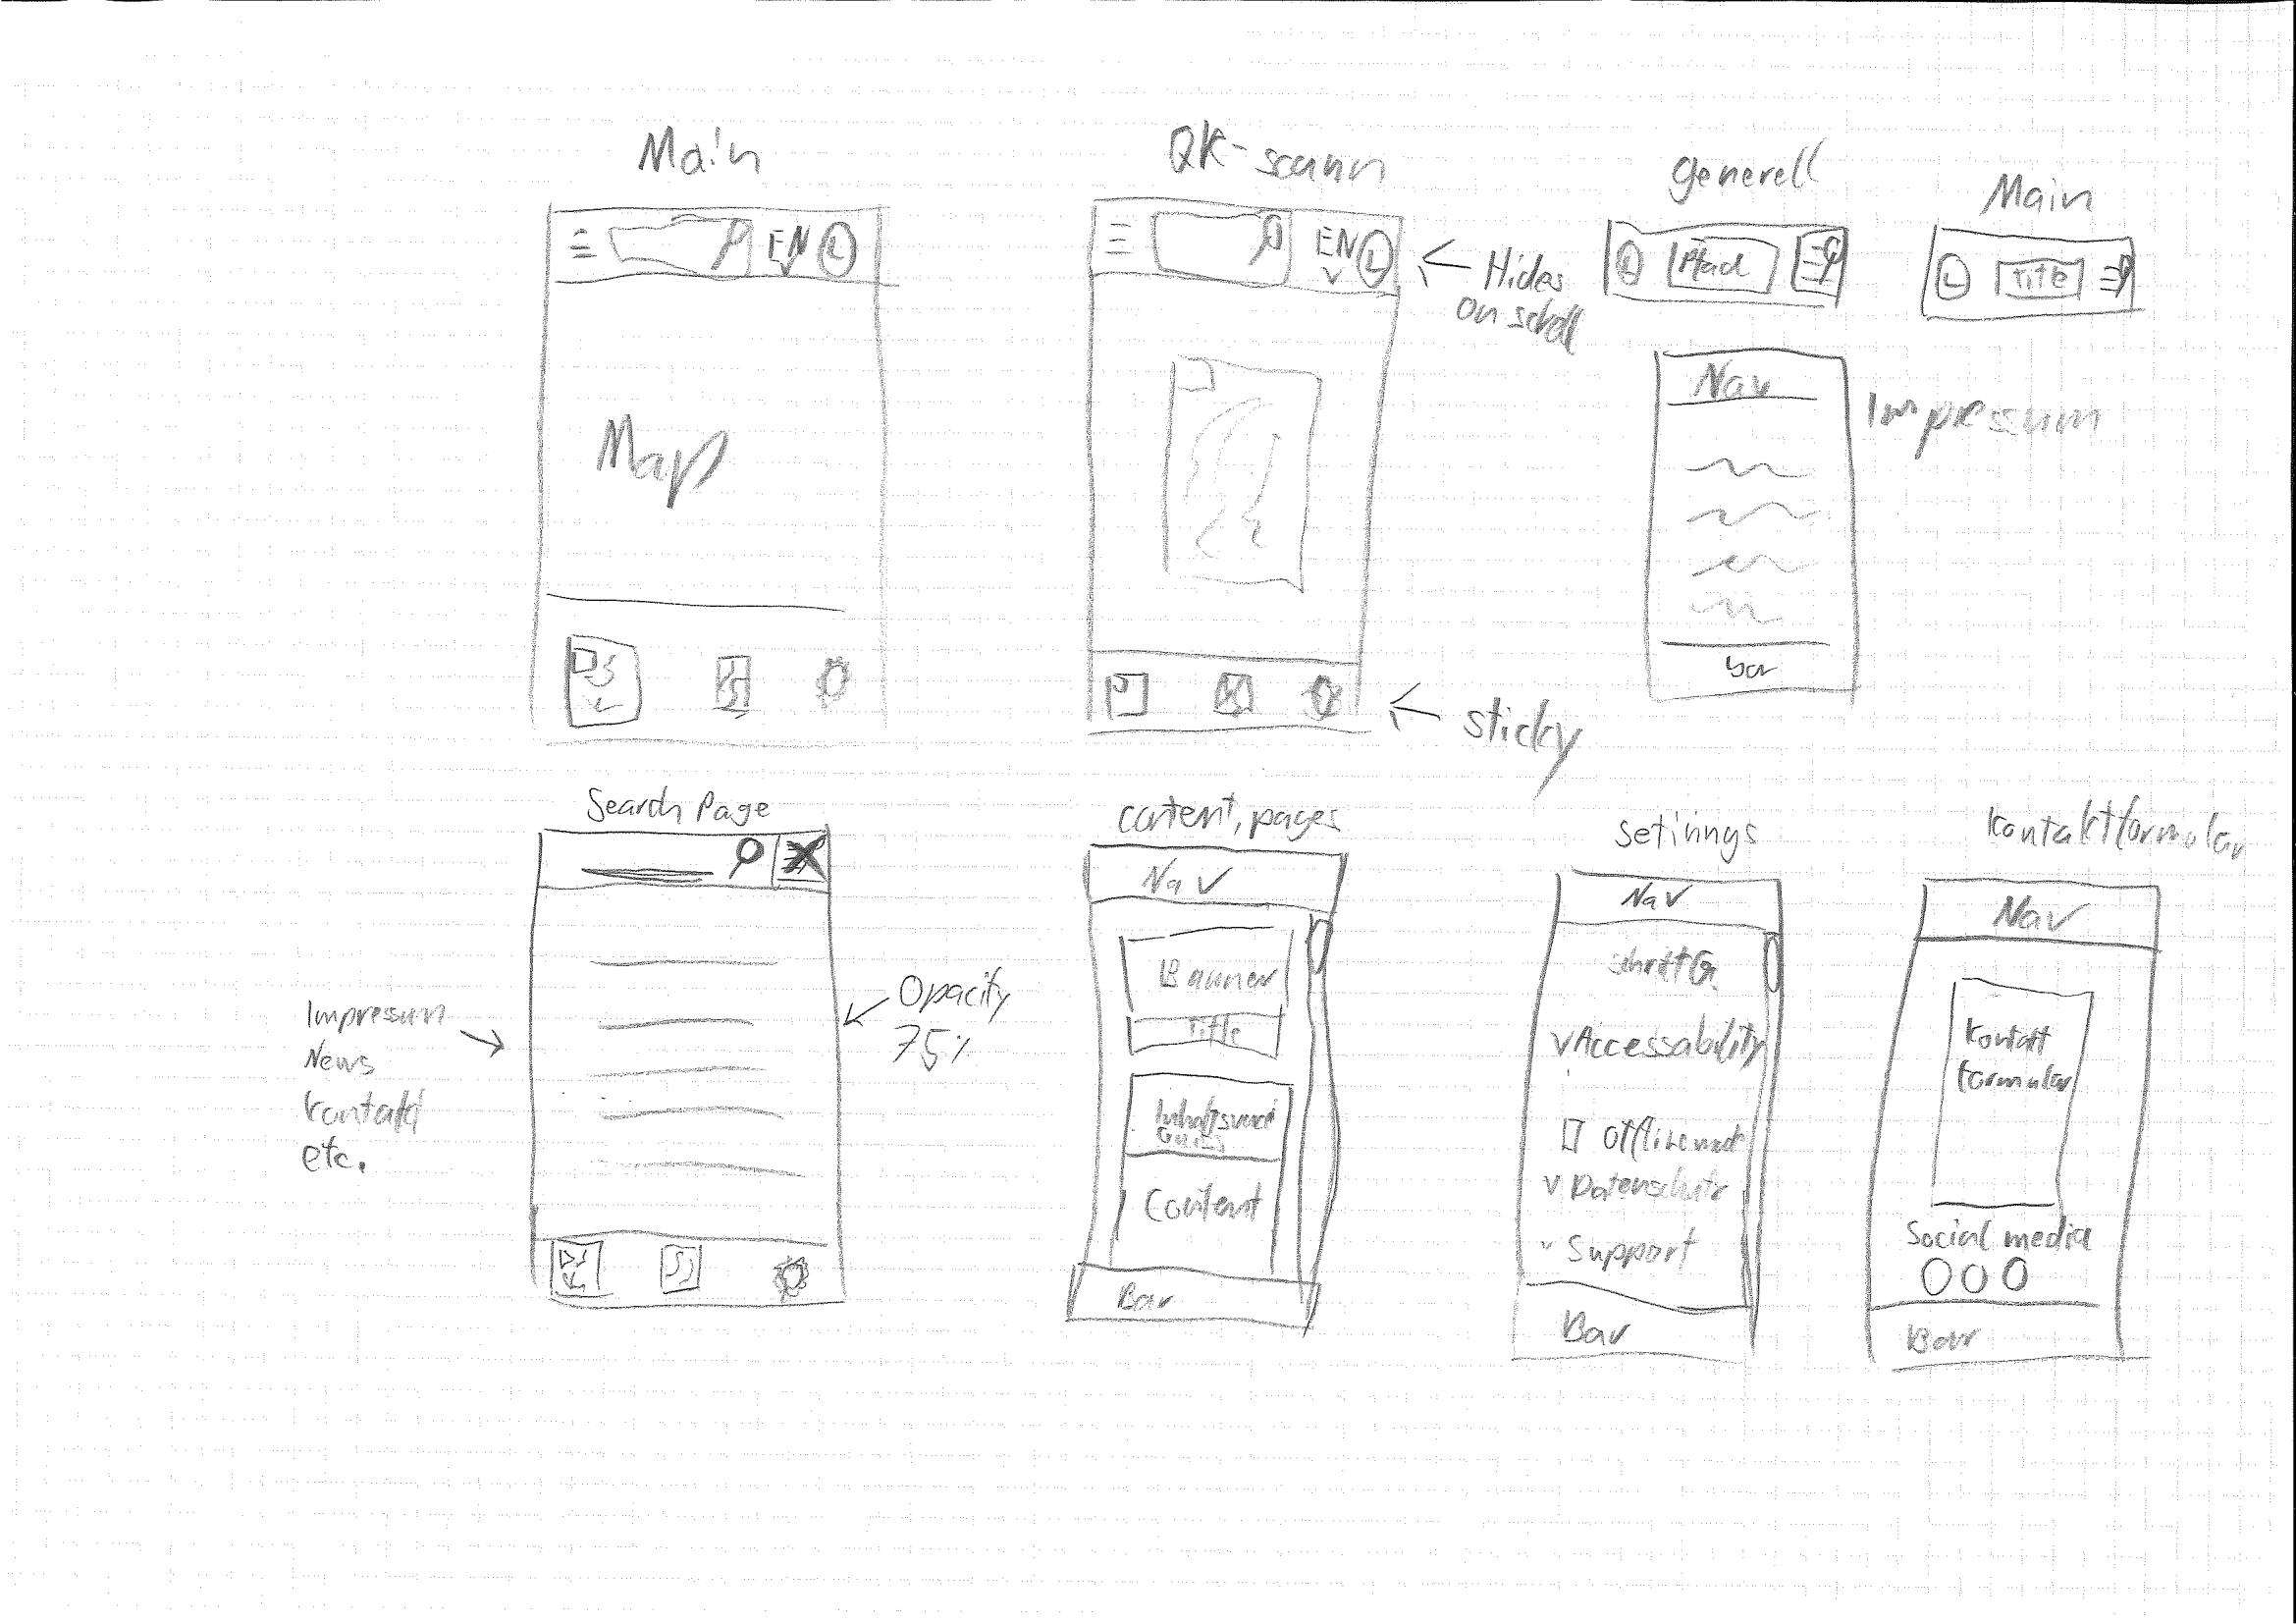
\includegraphics[width=17cm]{scribles-2-1}
	\\Wir legen unseren Fokus auf die Hauptseite hier als Main gekennzeichnet.\\
	Wir starteten mit einer simplen Navbar welche aus 4 Teilen besteht.
	\begin{itemize}
		\item Burgermenu:\\
		Welches eine Seite mit allen möglichen Weiterleitungen zu den Kontaktinformationen, Impressum, feedbackmöglichkeiten, etc. öffnet.
		\item  Suchfeld:\\
		Welches für das suchen der Einzelnen Atraktionen oder Kategorien gebraucht werden kann.
		\item Dropdwon Spracheinstellungen:\\
		Es sollen Deutsch, Englisch, Französich und Italensich zur verfügung stehen.
		\item  Logo:\\
		Zum Schluss fügten wir noch ein Logo welches auch als home Button agieren sollte hinzu.
	\end{itemize}
	Der Haupttil der Seite wird von der Karte des Areals verwendet. Diese Karte sollte interaktiv sein damit man schnell sehen kann wo man ist und wo man hin will.\\
	
	Unten haben wir eien Footer mit drei Knöpfen.
	\begin{itemize}
		\item QR-Code scanner:\\
		Leitet einen weiter auf die QR-Code scanner Seite
		\item  Karte:\\
		In der Mitte und als standard ausgewählt ist die Karte.
		\item Einstellungen:\\
		Alle relevanten einstellungen für die Applikation, wie Darkmode oder ein Screenreader.
	\end{itemize}
	
	\subsubsubsection{Benutzerschnitstellen Optimieren}
	Nach dem Initialen Design haben wir uns Inspiration bei bereits bestehenden Seiten geholt , eine davon war SRF. Dadurch haben wir uns entschieden unsere Navbar neu zu gestalten.\\
	Wir haben nach user Logo nach Links verschoben, da das eher typisch ist, und aus dem gleichen grund haben wir user suchfeld ganz nach rechts verschoben. Da Suchfeld und das Burgermenu wurden zu einen und zeigen beim ancklicken die als "Search Page" gekenzeichnete seite. In der Mitte der Navabar wird es neu auch immer eine "Breadcrumb Navigation" geben, um die Steuerbarkeit der Applikation zu erhöhen.\\
	
	Diese Kleinen änderungen nach einer bekannten Webseite sollte das verwenden der Webseite für neue User erleichtern, da sie bereits erfahrung mit ähnlichen Webseitenn haben können.
	
	
	\subsection{Eingabeformate kennzeichnen}
	\subsubsection{Einleitung}
	Bei uns gibt es nicht viel, was der Benutzer ausfüllen muss. Momentan ist das Kontaktformular das einzige. Deshalb werde ich mich in diesem Kapitel darauf konzentrieren. Beim Kontaktformular muss man den Namen, Vornamen, die Email Addresse und den Text eingeben.\\
	Das Kontaktformularist ein sehr einfaches Formular. Trotzdem muss es intuitiv sein. Die erwarteten Eingaben müssen klar sein. Z.\,B. beim Namen wird ein Wort erwartet. Das Feld muss ausgefüllt werden.
	\subsubsection{Pflichtfelder}
	Pflichtfelder gibt es bei praktisch allen Formularen. Meistens sind diese mit einem * markiert. Dieser ist oft rot, damit er besser sichtbar ist. So würde ich es auch hier machen.\\
	Damit es für alle klar verständlich ist, werde ich auch zu oberst im Formular schreiben, dass alle Pflichtfelder mit einem Stern (*) markiert sind.\\
	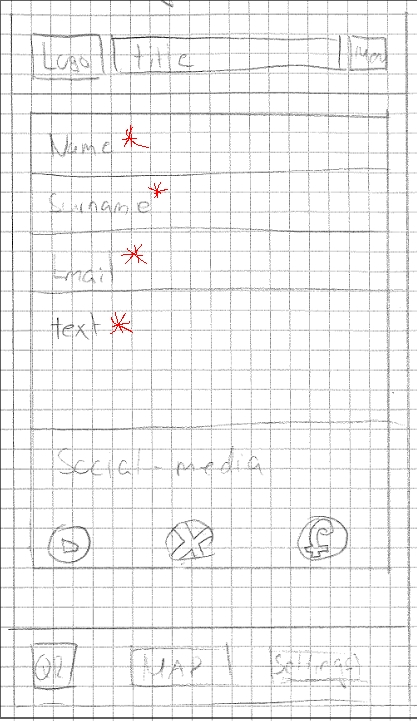
\includegraphics[width=5cm]{required-fields.jpg}
	\subsubsection{Eingabeformate}
	Falls sich der Benutzer im Internet nicht auskennt, kann es verwirrend sein, was bei den Feldern erwartet wird. Deshalb muss das klar erkennbar sein.\\
	Ich denke, dass es am einfachsten verständlich ist, wenn man einen Passenden Platzhalter für jedes Feld macht. Dabei soll der Platzhaltertext gräulich sein, damit man erkennt, dass es nicht Text ist, der wirklich ins Eingabefeld geschrieben ist.\\
	Als Platzhalter würde ich eine mögliche Eingabe nehmen. Beim Email Feld könnte das z.\,B. \textit{max.mustermann@example.com} sein.
	\subsubsection{Felder im Detail}
	Den Namen würde ich mit einem roten Stern kennzeichnen. Als Platzhalter würde ich Mustermann nehmen.\\
	Beim Feld für den Vornamen würde ich auch einen Stern platzieren. Statt Mustermann würde ich dann Max verwenden.\\
	Das Email Feld habe ich oben schon als Beispiel verwendet. Dieses würde ich auch mit einem Stern markieren und wie schon gesagt als Platzhalter \textit{max.mustermann@example.com} verwenden.\\
	Für den Text (die Nachricht) würde ich auch einen Stern verwenden. Als Platzhalter würde ich «\textit{Ihre Nachricht hier}» verwenden.
	
	\pagebreak
	
	\subsection{Hilfe und Feedback integrieren}
	
	\subsubsection{Feedback für User aktionen}
	
	Ziel: User informieren dass die Anwendung auf ihren Input reagiert.
	
	\begin{itemize}
		\item Erfolgs Nachricht
			\subitem Nach Formular abgabe
				\subsubitem "Deine Änderungen wurden gespeichert"
				\subsubitem \textit{(Bestätigung der erfolgreichen Verarbeitung von Nutzereingaben)}
		\item Fehlermeldungen
			\subitem Fehlende Felder in Formular
				\subsubitem "Bitte fülle alle mit einem * Markierten Felder aus"
				\subsubitem \textit{(Klare Kennzeichung von Pflichtfeldern gemäss ISO 9241-110)}
			\subitem E-Mail Validierung fehlgeschlagen
				\subsubitem "Invalides E-Mail Format. Beispiel: user@example.com"
				\subsubitem \textit{(Formatvorlge zur sofortigen Fehlerbehebung)}
		\item Ladeanzeiger / Animationen
			\subitem Datenabfragen
				\subsubitem Loading Spinner / Wheel
				\subsubitem \textit{(Visuelles Feedback bei kurzen Wartezeiten <3s)}
			\subitem File upload
				\subsubitem Progress Bar
				\subsubitem \textit{(Prozentuale Anzeige für längere Prozesse)}
			\subitem Kontent Ladescreen
				\subsubitem Skellet-Screen (normaler screen ohne Daten)
				\subsubitem \textit{(Wahrung des Aussehens und Format während des Ladens)}
	\end{itemize}
	
	Wir haben uns hier dafür entschieden eine Erfrolgsnachricht anzuzeigen wenn das Kontakt Formular abgesendet wird, die Felder Validierung einzu arbeiten und beim ersten starten der App eine Progressbar damit der User weiss wie schnell die Daten runter geladen werden.
	
	\subsubsection{Hilfefunktionen}
	
	Ziel: Benutzer unterstützen, falls sie unsicher sind, wie das Kontaktformular ausgefüllt werden soll.
	
	\begin{itemize}
		\item Platzhaltertext in Eingabefeldern
			\subitem Beispiel für das "Name"-Feld:
				\subsubitem \texttt{"Max Mustermann"}
			\subitem Beispiel für das "Betreff"-Feld:
				\subsubitem \texttt{"Betreff meiner Nachricht"}
				\subsubitem \textit{(Führt den Nutzer durch implizite Beispiele)}
		
		\item Automatische Vorschläge
			\subitem Bei der "E-Mail"-Eingabe:
				\subsubitem \texttt{"Meinten Sie: example@domain.com?"}
				\subsubitem \textit{(Typos erkennen durch Domain-Check)}
	\end{itemize}
	
	Wir werden hier beides implementieren um die UX der User zu verbessern.
	
	\subsubsection{Erweitertes Feedback}
	
	Ziel: Für eine Polierte UI, um Hilfe und Feedback dynamisch zu kombinieren.
	
	\begin{itemize} 
		\item Real-time validation
			\subitem zBs. Passwort Stärke Messer
		\item Rückgänig machen Option
			\subitem zBs. Wenn man eine Formular Sende Bestätigung bekommt, das man diese inerhalb von 5s noch zurück ziehen kann.
		\item Interaktives Tutorial
			\subitem zBs. Ein Step-by-step popup für neue Nutzer
	\end{itemize}
	
	Auch hier würden wir alles implementieren da es für die Nutzer die beste experience gibt.
	
\end{document}